\documentclass{../iot-lecture}

\subtitle{NS3 Simulation}

\begin{document}

\begin{frame}
  \titlepage{}
\end{frame}
\begin{frame}
  \frametitle{Outline}
  \tableofcontents{}
\end{frame}

\section{Introduction}

\begin{frame}
  \frametitle{NS3}
  \begin{itemize}
    \item Discrete-event Simulator
    \item Typically run from command line
    \item Written in C++, not in a high-level modeling language
  \end{itemize}
\end{frame}

\begin{frame}
  \frametitle{NS3 (Cont'd)}
  \begin{itemize}
    \item The \textit{\color{YellowOrange} main()} program is where the specific simulation scenario configuration
      is performed and where the simulator is run and stooped.
    \item Most users end up editing and having to rebuild the \textit{ns-3} libraries themselves,
      so having the source code available is more convenient.
  \end{itemize}
\end{frame}

\begin{frame}
  \frametitle{NS3 Installation}
  \begin{itemize}
    \item Most beginning users need not concern themselves if their configuration reports some missing
      optional features of \textit{ns-3}.
  \end{itemize}
  \begin{table}
    \begin{tabular}{cp{.7\textwidth}}
      Prerequisite &
      Package/Version \\

      C++ compiler &
      \textit{clang++} or \textit{g++} (g++ version 7 or greater) \\

      Python &
      \textit{python3} version $\geq$ 3.6 \\

      Git &
      any recent version (to access \textit{ns-3} from \href{https://github.com/nsnam/ns-3-dev-git}{Github.com}) \\

      tar &
      any recent version (to unpack an ns-3 release) \\

      bunzip2 &
      any recent version (to uncompress an ns-3 release) \\
    \end{tabular}
  \end{table}
\end{frame}

\begin{frame}[fragile]
  \frametitle{NS3 Installation (Cont'd)}
  \scriptsize
  \begin{minted}{console}
> cd
> mkdir workspace
> cd workspace
> wget https://www.nsman.org/release/ns-allinone-3.35.tar.bz2
> tar xjf ns-allinone-3.35.tar.bz2
  \end{minted}
\end{frame}

\begin{frame}[fragile]
  \frametitle{First Network}
  \scriptsize
  \begin{minted}{cpp}
using namespace ns3;

int main(int argc, char *argv[]) {
  Time::SetResolution(Time::NS);

  NodeContainer nodes;
  nodes.Create(2);

  PointToPointHelper pointToPoint;
  pointToPoint.SetDeviceAttribute("DataRate", StringValue("5Mbps"));
  pointToPoint.SetChannelAttribute("Delay", StringValue("2ms"));

  NetDeviceContainer devices;
  devices = pointToPoint.Install(nodes);

  InternetStackHelper stack;
  stack.Install(nodes);

  // ...

  Simulator::Run();
  Simulator::Destroy();
  return 0;
}
  \end{minted}
\end{frame}

\begin{frame}
  \frametitle{Use Linux Containers to set up virtual networks}
  \begin{figure}
    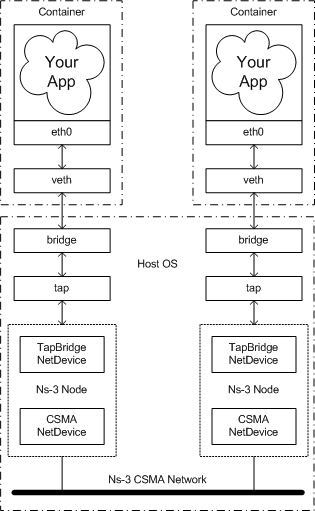
\includegraphics[height=.8\textheight]{./img/container_and_ns3_bd.png}
  \end{figure}
\end{frame}

\begin{frame}
  \frametitle{Use Linux Containers to set up virtual networks (Cont'd)}
  \begin{itemize}
    \item The dotted-dashed lines demark the containers and the host OS\@.
    \item These net devices are actually connected to Linux bridges that form the connection to the host OS\@.
    \item  There is a tap device also connected to each of these bridges.
    \begin{itemize}
      \item These tap devices bring the packets flowing through them into user space where ns-3 can get hold of them.
      \item A special ns-3 NetDevice attaches to the network tap and passes packets on to an ns-3 \textbf{ghost node}.
    \end{itemize}
  \end{itemize}
\end{frame}

\section{LoRaWAN}

\begin{frame}
  \frametitle{An ns-3 module for simulation of LoRaWAN networks}
  \begin{itemize}
    \item \href{https://github.com/signetlabdei/lorawan}{Website}
    \item Current features include:
    \begin{itemize}
      \item Support for Class A devices
      \item Network Server Implementation
      \begin{itemize}
        \item ADR
        \item Confirmed messages
        \item Multi-GW support
      \end{itemize}
      \item Urban propagation models
      \item Realistic GW chip model
      \item Energy model integration
    \end{itemize}
  \end{itemize}
\end{frame}

\end{document}
